La première des alertes que nous proposons de traiter est l'alerte
dite du \emph{Grand Veymont,} issue de l'enregistrement d'un appel au
secours effectué XXXXX par un accompagnateur en montagne, au sujet
d'un de ses clients.

\subsection{Présentation de l'alerte}
\label{subsec:9-2-1}

Cette alerte est la plus courte de celles que nous présenterons ici,
elle est composée de 12 extraits, pour un total de 16 \emph{indices de
  localisation.}



Pas d'objets multiples

les indications données par le requérant sont assez précises et
détaillées, il est donc possible de définir une \emph{zone initiale de
  recherche} de petite taille. Nous avons défini une \ac{zir} de
\SI{25}{\kilo\meter\squared} (\autoref{fig:zir_grand_veyont}).

\begin{figure}
  \centering
  \begin{tikzpicture}
  \tikzset{et/.style={above,font=\footnotesize\vphantom{Ag}}}
  %
  \node[inner sep=0pt, anchor=south west] (image) at (0,0){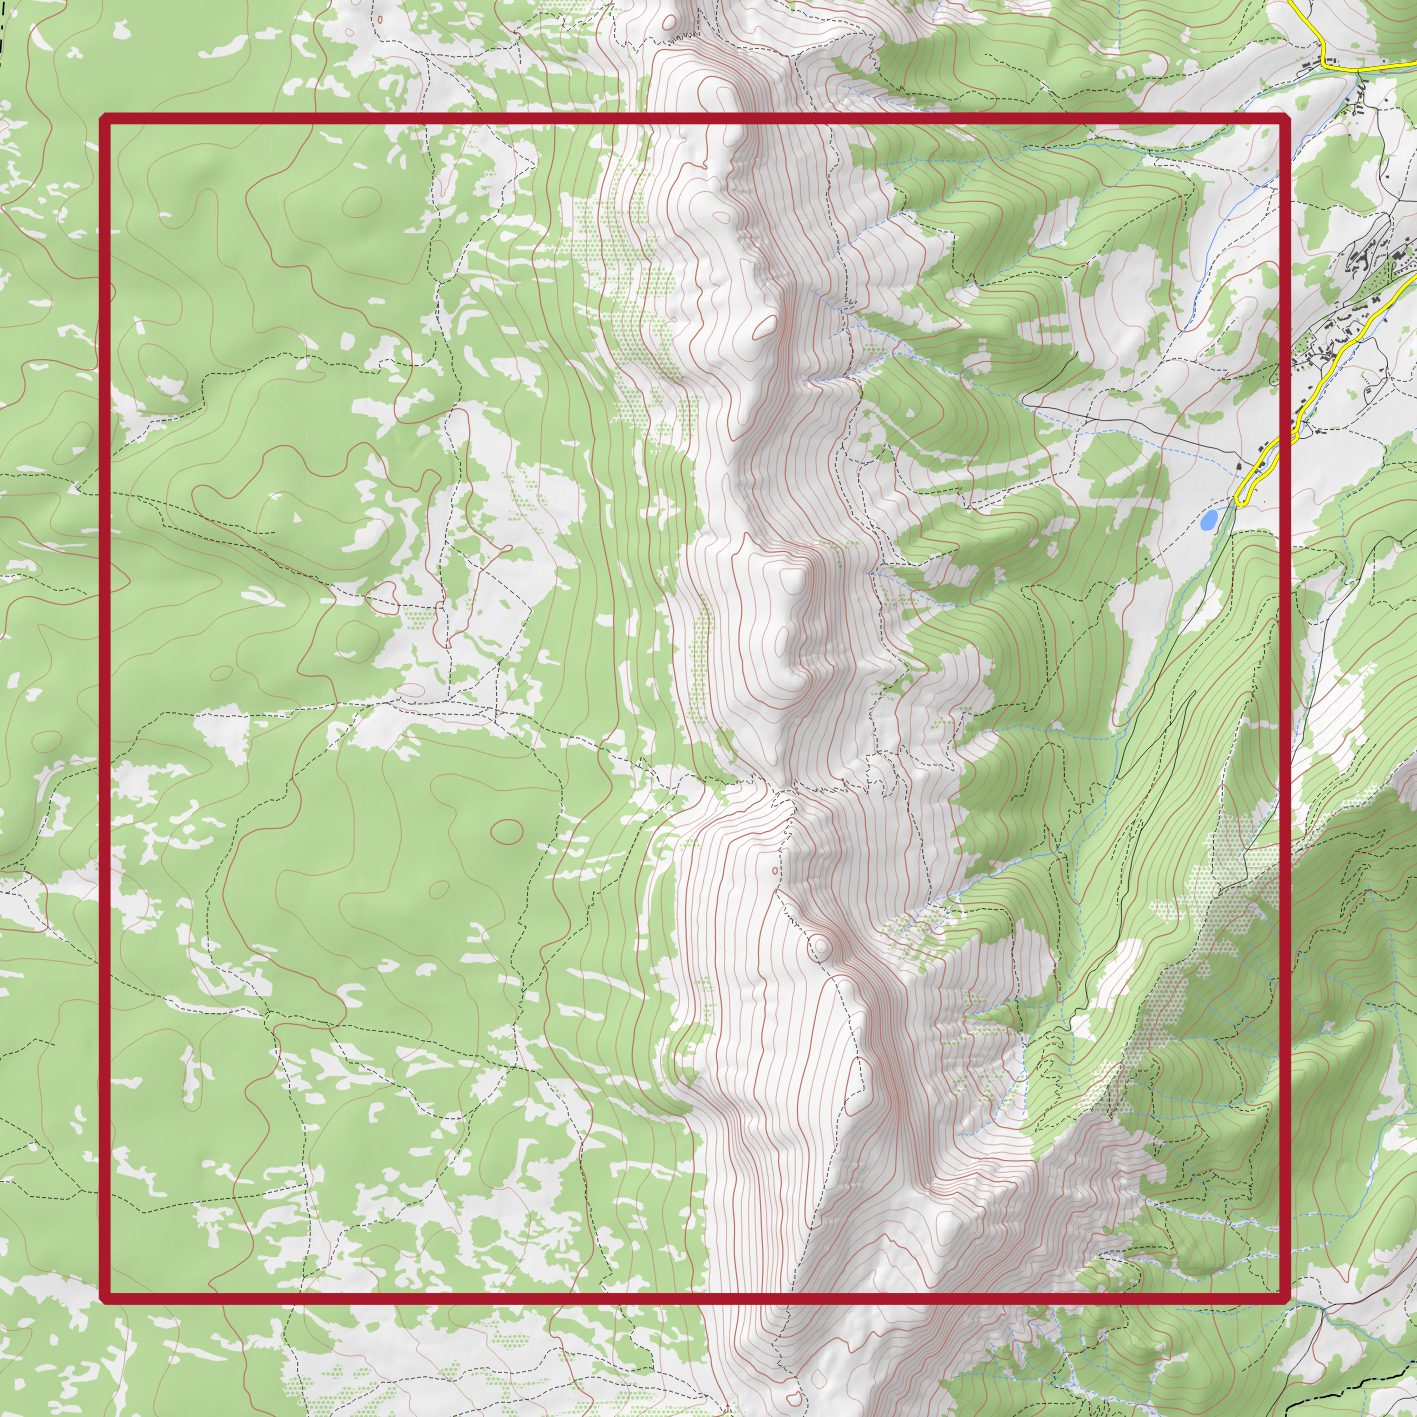
\includegraphics{./figures/ZIR_grand_veymont.png}};
  %
  \begin{scope}
    \node (P2) at ([yshift=-.5cm]image.south east) {};
    \node (P1) at ([yshift=-.5cm]image.south west) {};
    %
    \foreach \x [evaluate=\xshift using \x/10, evaluate=\rad using (\x * .0004) + .01] in {0,...,100}
    {
      \draw[fill=black,draw=none, below] ([xshift=\xshift cm, yshift=-.5cm]P1) circle [radius=\rad cm];
    }
    %
    \path(P1 |- 0cm,-1cm) --++ (10,0)
    node[et,pos=0] {0}
    node[et,pos=.1] {0,1}
    node[et,pos=.2] {0,2}
    node[et,pos=.3] {0,3}
    node[et,pos=.4] {0,4}
    node[et,pos=.65] {0,65}
    node[et,pos=1] {1};
    % Échelle
    \draw[-] (P2 |- -1cm,-1cm) --++ (-1,0) node[et,pos=.5] {\SI{500}{\meter}};
    % Légende détaillée
    \path (P1) -- (P2) node[pos=.5, yshift=-1cm] {\tiny Pour la légende détaillée du fond topographique voir \autoref{anx:topo_leg}. Sources: BD TOPO 2018, BD ALTI 2018.}; 
  \end{scope}
\end{tikzpicture}
  \caption{Zone initiale de recherche pour l'alerte \enquote{Grand Veymont}}
  \label{fig:zir_grand_veyont}
\end{figure}


\subsubsection{Retranscription et identification des indices de localisation}
\label{subsec:9-2-1-1}


Le verbatim de l'enregistrement audio de l'alerte \emph{Grand Veymont}
est donné dans la \autoref{anx:retrans-gv-verb}.
%
Comme nous l’expliquions dans le \autoref{chap:05}, 


Une partie des indices retranscrits ne sont cependant pas pertinents
pour notre cas d'appliqaution.

% Entre Grand Veymont et pas de la ville
% Je ne suis pas sur le sommet
% Je suis sous le grand Veymont
% Côté Sud/Nord

% Au dela

% not foret

% 800


\subsection{Modélisation de l'alerte}
\label{subsec:9-2-2}


\subsubsection{Décomposition des indices des indices de localisation}
\label{subsec:9-2-2-2}

\subsubsection{Spatialisation des indices de localisation décomposés}
\label{subsec:9-2-2-3}

\subsubsection{Fusion des zones de localisation compatibles}
\label{subsec:9-2-2-4}

À la suite de la spatialisation des différents indices de localisation
on dispose de plusieurs \ac{zlc}, qu'il est nécessaire de fusionner.

Seul un indice de localisation 


\subsection{Critique de la modélisation}
\label{subsec:9-2-3}

\tdi{Impact de la position du toponyme "pas de la ville" sur la modélisation}

%%% Local Variables:
%%% mode: latex
%%% TeX-master: "../../../../main"
%%% End:
